\subsection{Random Forest}

En aquesta secció s'explicarà el desenvolupament del mètode de \textit{Random Forest}\cite{randomForestlibrary}. Per a trobar el nombre d'arbres adequat pel nostre conjunt de dades s'ha usat diferents nombres d'arbres entre 50 i 1000 per entrenar i s'ha escollit el nombre d'arbres que dóna un \textit{Out-of-bag} menor. En la figura~\ref{fig:OOB} es pot observar l'evolució del nombre de \textit{Out-of-bag}, nombre d'errors, en funció del nombre d'arbres usat. S'aconsegueix l'error més petit usant 900 arbres amb un encert d'entrenament del 96.1\%.

\begin{figure}[H]
    \centering
    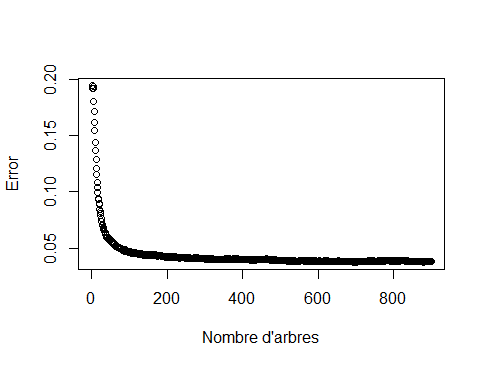
\includegraphics[width=0.8\textwidth]{img/randomPlot.png}
    \caption{Evolució del nombre de \textit{Out-of-bag}}
    \label{fig:OOB}
\end{figure} 

Un avantatge que ofereix el mètode de \textit{Random Forest} és que mostra la importància de cada variable en el model. Com es pot observar en la figura~\ref{fig:imp} la variable més important en el nostre model és la número 14, la qual correspon al número mitjà d'arestes de dreta a esquerra. Per l'altre banda, la variable menys important correspon a la número 5, l'alçada de la capsa a on és la figura.

\begin{figure}[H]
    \centering
    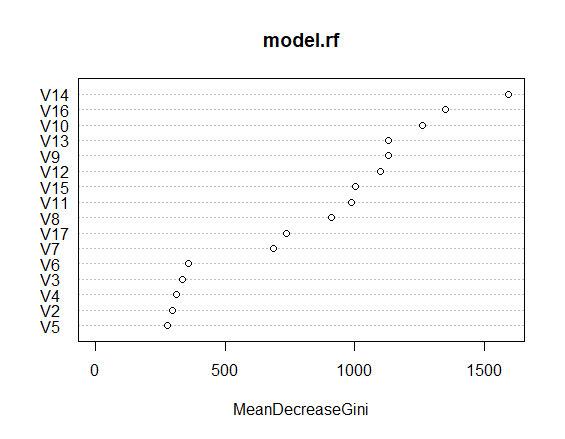
\includegraphics[width=0.8\textwidth]{img/importanceRF.png}
    \caption{Importància de cada variable}
    \label{fig:imp}
\end{figure}

El model aconsegueix un 96.27\% d'encert en el conjunt de dades de prova. També el model obté un 0.9847 de \textit{F1 score} aquest valor tan pròxim a 1 indica que la distribució de la predicció està ben balancejada entre les 26 classes diferents. 
